\subsection{Login}
When a user visits the website, they need to decide between logging in using their Feide account or continue as an anonymous user. At this stage, their user-rights level is set to 0, and they can only access the login page. Anonymous users have a user-rights level of 1 and can participate in sessions. If the user authenticates with their Feide account, they are assigned a user-rights level depending on their admin status. A regular user with no special rights will get their level set to 2. Level 3 is used for student assistants. Admins (lecturers, professors, ...) are assigned level 4. Users with a user-rights level above 1 can see statistics about sessions they have participated in. Student assistants and admins can create, edit and delete questions and sessions. They can also host a session. Admins can create courses. They are also able to add and remove admins and student assistants to a course. A user with admin or student assistant privileges can apply to get a role in another course. Only admins for that course can accept or decline the request.
\subsubsection{Implementation}
\begin{figure}[H]
    \centering
    \begin{subfigure}{0.45\linewidth}
        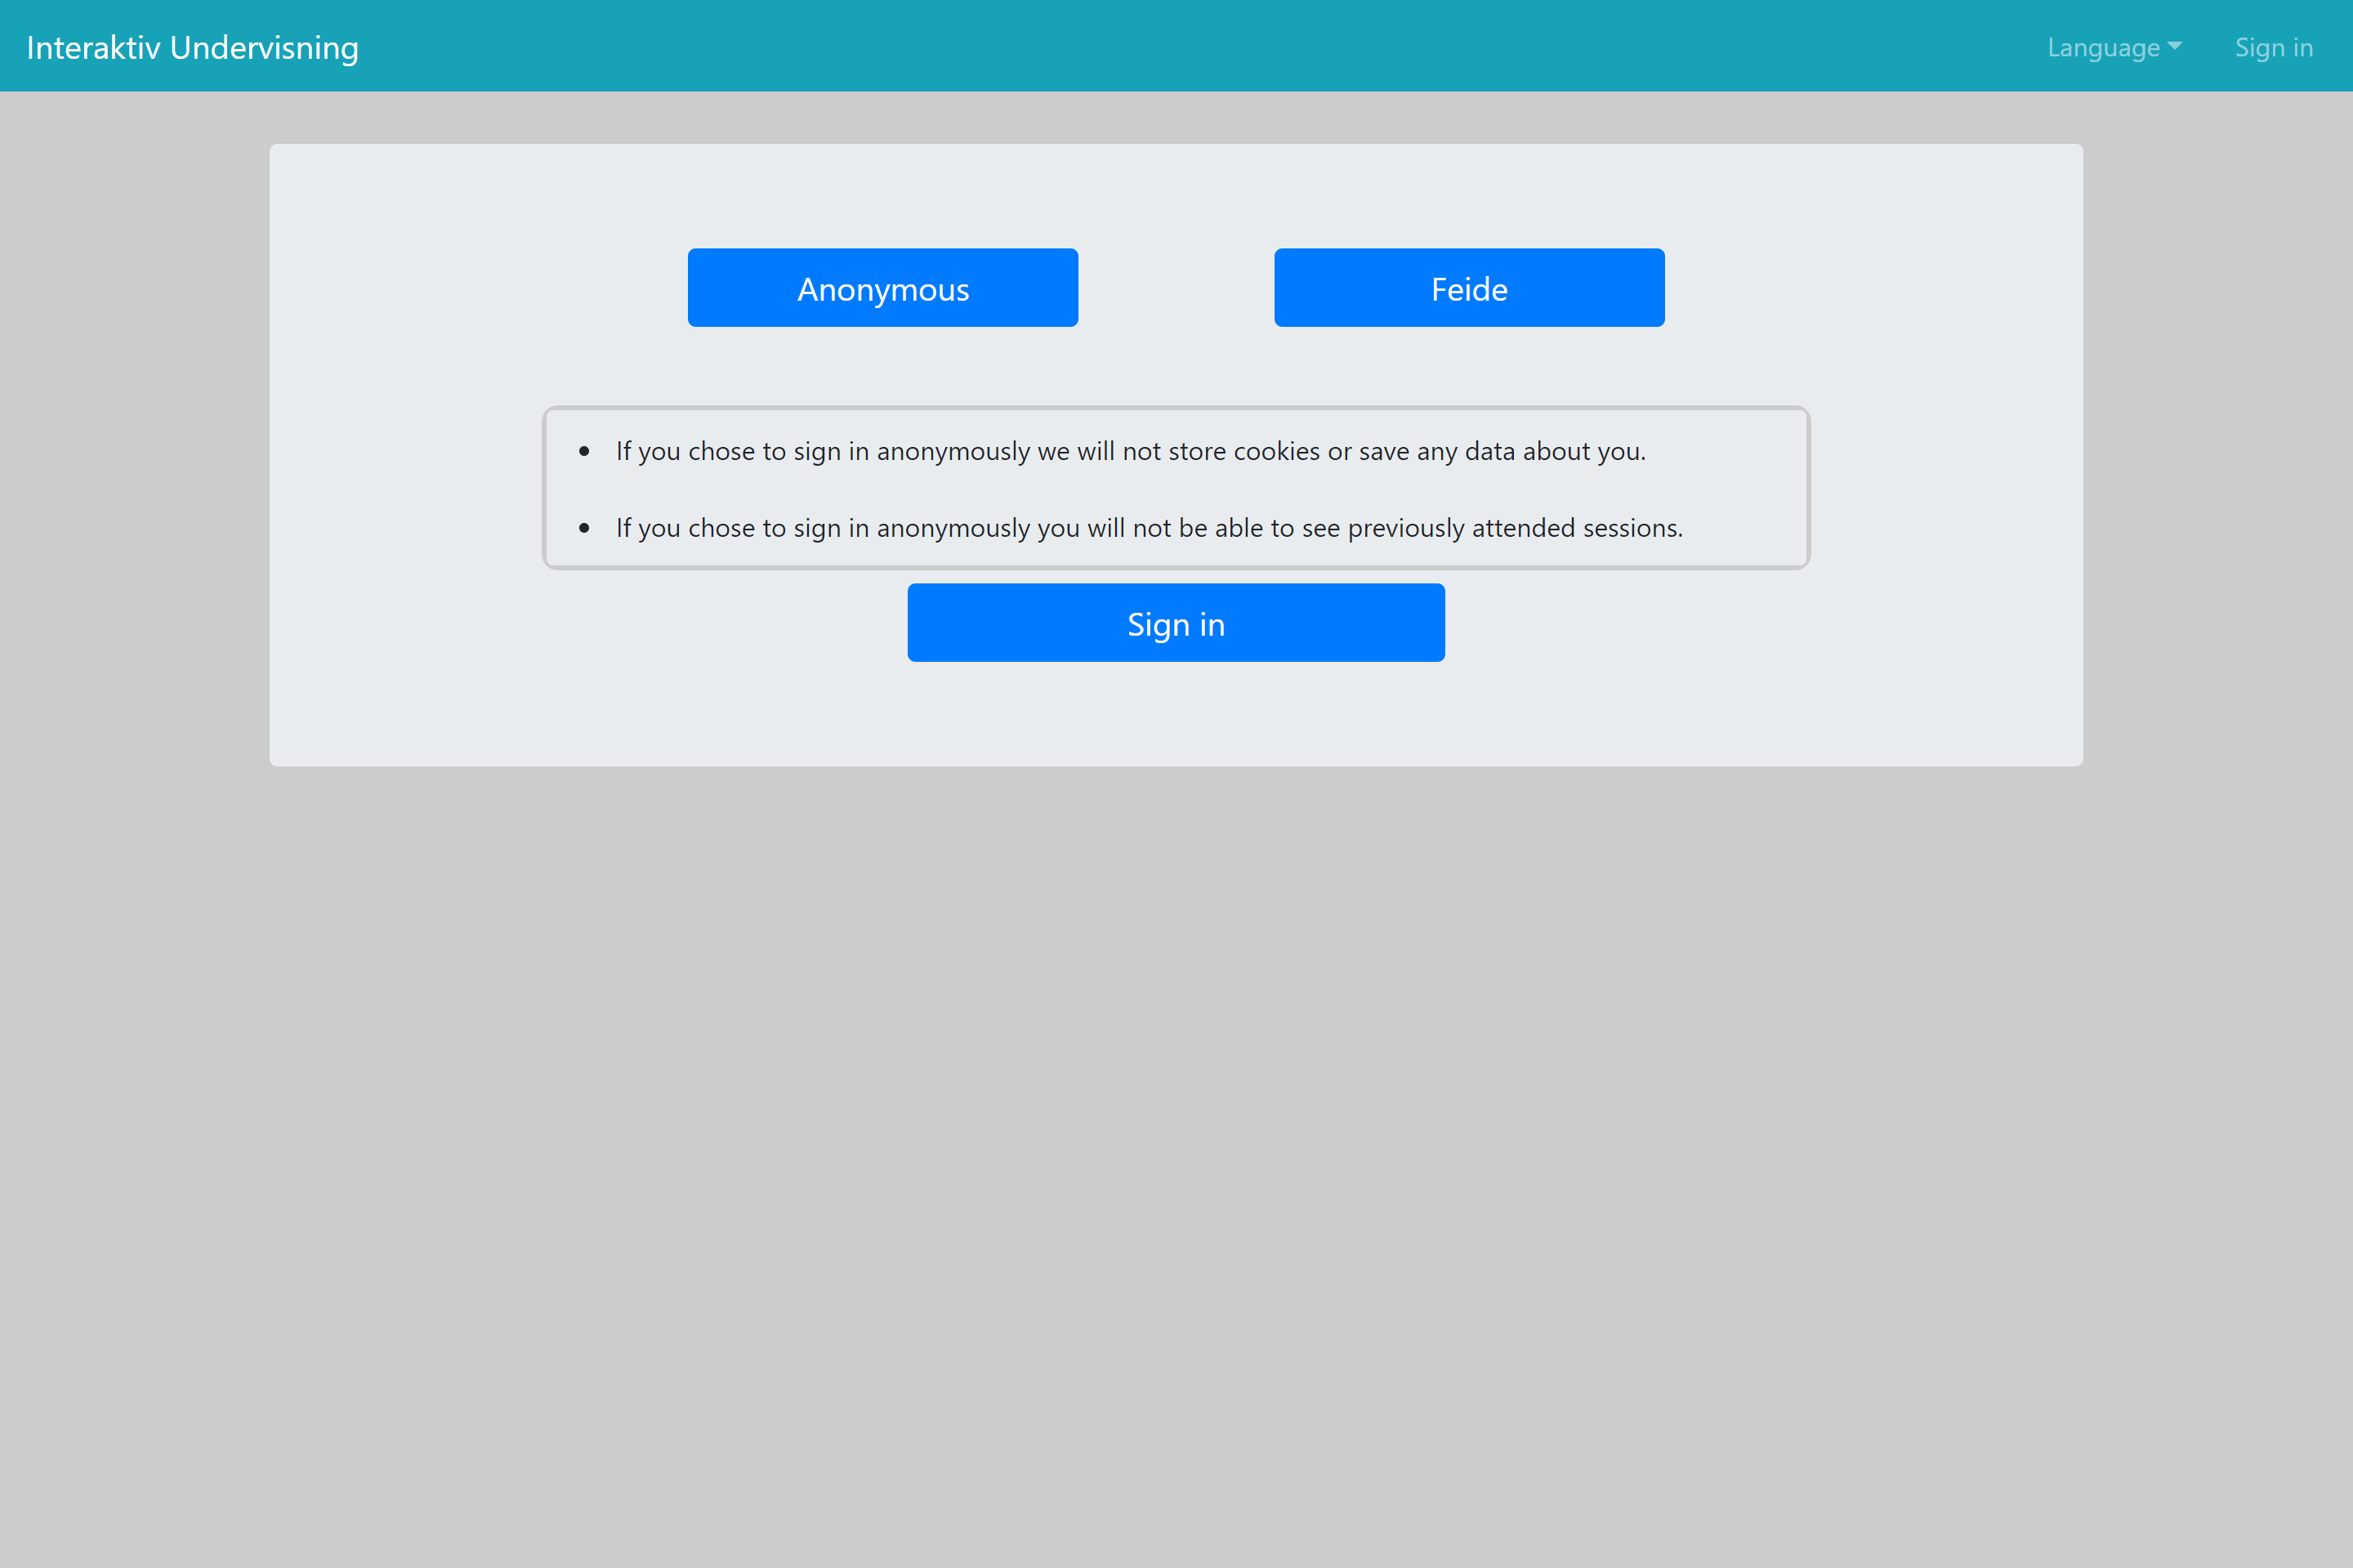
\includegraphics[width=\linewidth]{loginPageAnonymously}
        \caption{This is how the login page looks when anonymously is selected.}
        \label{fig:loginPageAnonoumsly}
    \end{subfigure}
    \begin{subfigure}{0.45\linewidth}
        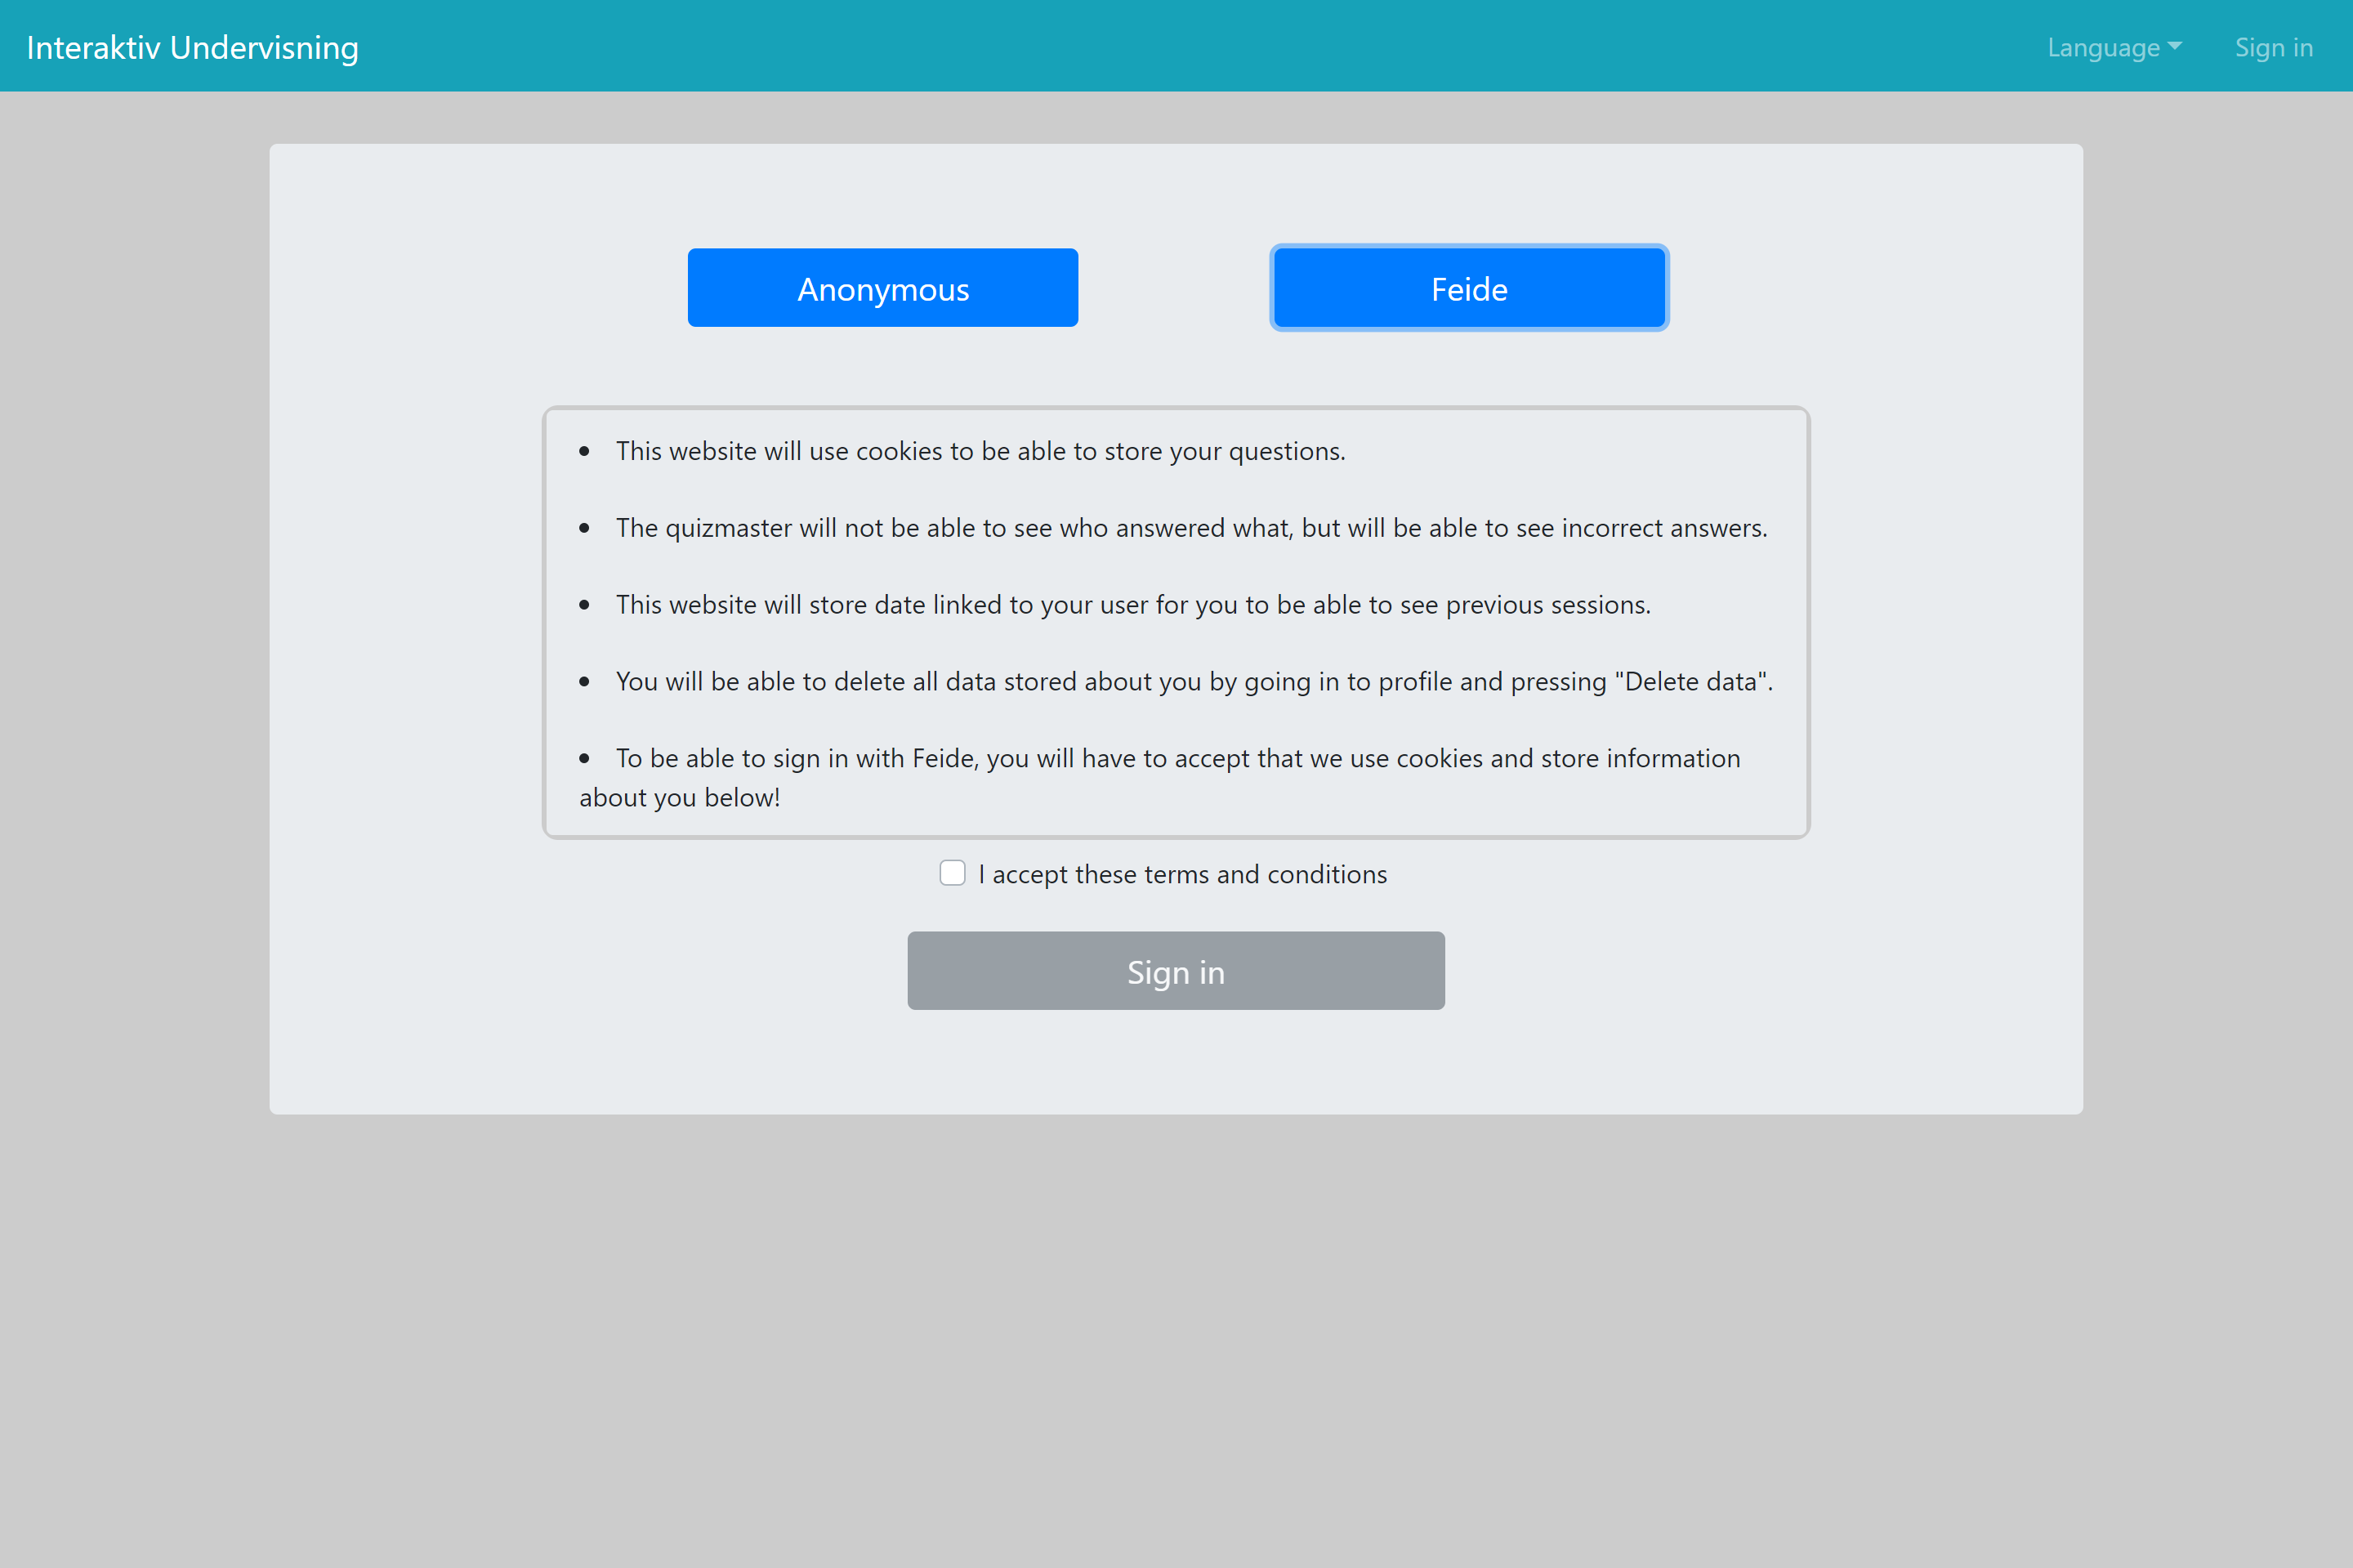
\includegraphics[width=\linewidth]{loginPageFeide}
        \caption{This is how the login page looks when feide is selected.}
        \label{fig:loginPageFeide}
    \end{subfigure}
    \caption{Login Page}
    \label{fig:loginPage}
\end{figure}
\noindent
If a user wants to be anonymous, their user-rights level is first set to 1. They are then redirected to the client page. Since it was decided that an anonymous user should not be tracked or have any information stored about them. They are limited to only clicking buttons on the page to navigate. Any attempts to reload the page or going directly to an URL results in the user getting redirected to the 401 error page indicating that the user is not authenticated to view this part of the web app. All answers that are sent in by an anonymous user is stored in the database for the lecturer to view. There is no link between the user and the answer given. Therefore, all answers from anonymous users link to the same user in the database.
\\[11pt]
If the user clicks on the Feide login button and accepts the terms, a HTTP POST request is sent to /login/feide. When the server receives the request, it is passed on to PassportJS's authenticate function. The authenticate function redirects the user to an external site for authentication, before redirecting them back to the specified callback URL on the application site. The authenticate function takes an argument telling it where and how to redirect the user; this is called a strategy. The /login/feide route uses the "passport-openid-connect" strategy to connect to Uninett's Dataporten authentication servers. If the user successfully logs in with their Feide account, they are redirected back to /login/callback/feide. This route uses the PassportJS authenticate function to exchange the access code with an access token which is then passed on to the route handler. The handler reads the HTTP request to get information about their Feide account. This information is used to check the database and create an in-memory user object which the server uses to decide what the user is allowed to do on the server. The user is finally redirected to the /client route where they can join a session. The server also sends a cookie for Feide users so that they will stay authenticated for one day, and during this time there is no need for the user to re-authenticate with Feide. When a Feide user signs out, the cookie is deleted. Since the web application is designed to be used on campus at UiS, users are stored in-memory when they are signed in and active on the web application, but this will result in problems if the application is scaled up to more users.
\\[11pt]
The way the database and the paths are designed it should be easy to add more sign in options for a user, such as Google, Facebook, etc. The way the user right system is designed, only Feide users can be admins or student assistants. When the server first starts the site will have zero admins, but there is a variable in the environment file where admins can be added. This bypasses the normal way to add an admin via the admin site.